\documentclass[12pt,a4]{article}
\usepackage[utf8]{inputenc}
\usepackage[portuguese,brazilian]{babel}
\usepackage[lmargin=3cm,tmargin=3cm,rmargin=2cm,bmargin=2cm]{geometry}
\usepackage[T1]{fontenc}
\usepackage{amsmath,amsthm,amsfonts,amssymb,dsfont,mathtools,blindtext}
\usepackage{graphicx}
\usepackage{booktabs}
\usepackage[dvipsnames]{xcolor}

\title{Relatório de Análise de Componentes}
\author{Gabriel Medina, Jonatas Fernandes}
\date{Junho 2023}

\begin{document}
\maketitle

\section{Introdução}
Neste relatório, será descrita uma análise de componentes principais (PCA) realizada em um conjunto de dados relacionados aos valores nutricionais de produtos do Starbucks. O PCA é uma técnica estatística que permite identificar padrões e estruturas nos dados, reduzindo sua dimensionalidade e facilitando a interpretação.

\section{Base de Dados}
O conjunto de dados utilizado neste estudo contém informações sobre alimentos do Starbucks e foi obtido através do site Kaggle.com. O arquivo CSV contém informações sobre calorias, gorduras e fibras dos alimentos.

\section{Codificação}
A codificação do algoritmo de Análise de Componentes Principais (PCA) foi implementada utilizando a linguagem de programação Python e as seguintes bibliotecas: NumPy para manipulação de arrays e realização de cálculos matemáticos, pandas para leitura e manipulação dos dados, e Matplotlib para a visualização gráfica.
\begin{flushleft}
Primeiramente, os dados são lidos de um arquivo CSV utilizando a biblioteca Pandas. Em seguida, são extraídas as colunas relevantes para a análise (Calories, Fat(g), Carb.(g), Fiber(g), Protein, Sodium). O algoritmo de PCA é aplicado utilizando a função "perform pca", que utiliza as bibliotecas NumPy para manipulação de arrays e cálculos matemáticos. A função retorna os dados projetados nos componentes principais.
\end{flushleft}

\begin{flushleft}
A visualização dos dados é realizada utilizando a biblioteca Matplotlib. Os pontos projetados nos componentes principais são plotados em um gráfico tridimensional, onde a cor de cada ponto representa a escala de valores da variável correspondente ao componente principal. O gráfico é configurado com rótulos nos eixos, título e uma legenda explicativa, por fim, o gráfico é exibido utilizando a função plt.show(), permitindo a visualização dos resultados da análise de componentes principais no conjunto de dados do Starbucks.
\end{flushleft}

\newpage
\section{Resultado}
A figura abaixo, gerada pelo código, apresenta uma representação tridimensional dos dados projetados nos três primeiros componentes principais.

\begin{center}
    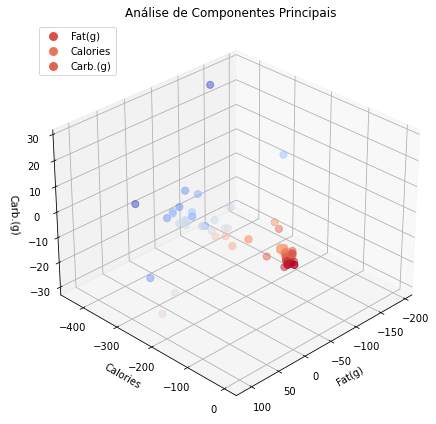
\includegraphics[scale=0.9]{1.png}
\end{center}

\begin{flushleft}
Cada ponto no gráfico representa um produto do Starbucks, e a cor do ponto indica a escala de valores da variável correspondente ao componente principal, azul indica valores baixos e vermelho indica valores altos.
\end{flushleft}

\end{document}